\documentclass[crop,tikz]{standalone}

\usepackage[utf8]{inputenc}
\usepackage{ifthen}

% 'crop' is the default for v1.0, before it was 'preview'
%\usetikzlibrary{...}% tikz package already loaded by 'tikz' option

%tikz structures and patterns
\usetikzlibrary{patterns}

%hexagon drawing variables
\def\ly{0.866025} %sin(pi/3) = sqrt(3)/2
\def\lx{0.5} %cos(pi/3) = 0.5
\def\hexSize{5} %size of the hexagon that'll be the extent of the fibre cross section
\def\coreSize{0.2} %size of hollow cores
\def\coreSep{0.5} %separation between core CENTRES HORIZONTALLY
\def\coreSepHeight{0.4464} %separation between core CENTRES VERTICALLY

\newcommand{\hexagon}[4]{
\begin{scope}[shift={#2}]
	\draw[#3, fill=#4] (-#1*\lx, #1*\ly) -- (#1*\lx, #1*\ly) -- (#1,0) -- (#1*\lx, -#1*\ly) -- (-#1*\lx, -#1*\ly) -- (-#1,0) -- cycle;
\end{scope}
} %\hexagon{centre-to-corner-length}{shift (x,y)}{line spec}{fill colour} [none is allowed for fillcolour]

  
\begin{document}

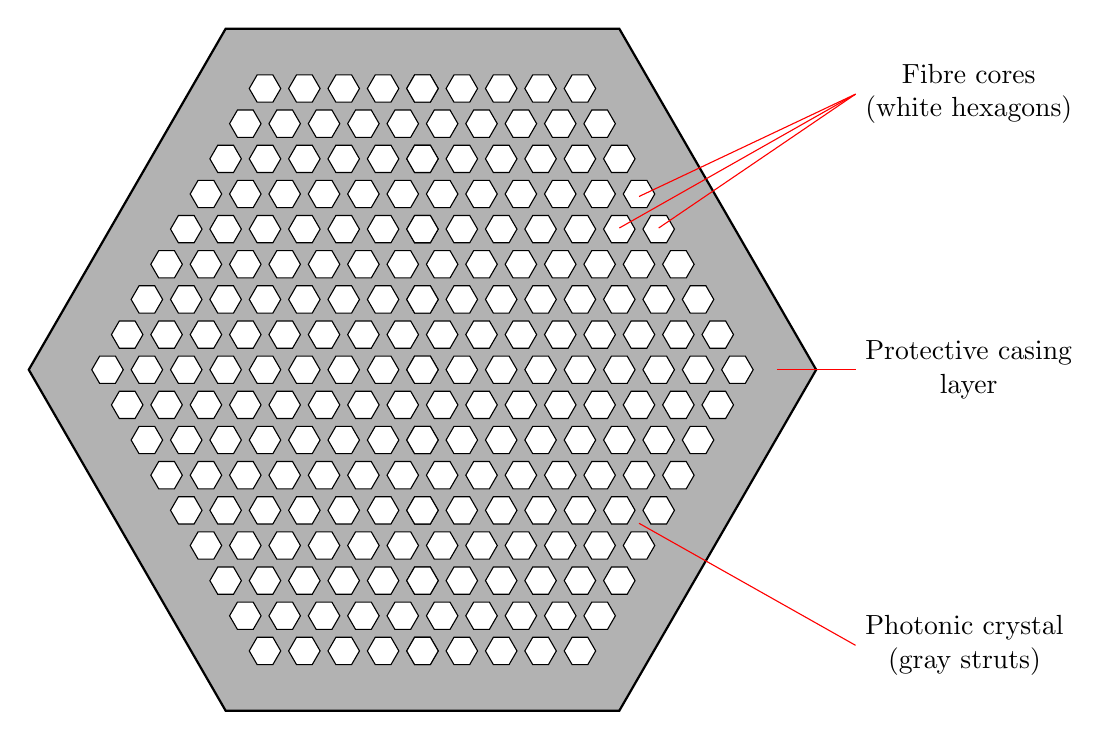
\begin{tikzpicture}

	%fibre outline
	\hexagon{\hexSize}{(0,0)}{thick}{black!30!white}
	
	%fibre cores using loopy loops, but because I can't get tikz to do basic arithmetic I've just written this out by hand for each lattice rack ... jokes
	\foreach \x in {0, ..., 8} %y=0
		\hexagon{\coreSize}{(\x*\coreSep,0*\coreSepHeight)}{}{white}
		\hexagon{\coreSize}{(-\x*\coreSep,0*\coreSepHeight)}{}{white}	
		; %end for \x
	\foreach \x in {0, ..., 7} %y=2
		\hexagon{\coreSize}{(\x*\coreSep,2*\coreSepHeight)}{}{white}
		\hexagon{\coreSize}{(-\x*\coreSep,2*\coreSepHeight)}{}{white}	
		\hexagon{\coreSize}{(\x*\coreSep,-2*\coreSepHeight)}{}{white}
		\hexagon{\coreSize}{(-\x*\coreSep,-2*\coreSepHeight)}{}{white}	
		; %end for \x
	\foreach \x in {0, ..., 6} %y=4
		\hexagon{\coreSize}{(\x*\coreSep,4*\coreSepHeight)}{}{white}
		\hexagon{\coreSize}{(-\x*\coreSep,4*\coreSepHeight)}{}{white}	
		\hexagon{\coreSize}{(\x*\coreSep,-4*\coreSepHeight)}{}{white}
		\hexagon{\coreSize}{(-\x*\coreSep,-4*\coreSepHeight)}{}{white}	
		; %end for \x
	\foreach \x in {0, ..., 5} %y=6
		\hexagon{\coreSize}{(\x*\coreSep,6*\coreSepHeight)}{}{white}
		\hexagon{\coreSize}{(-\x*\coreSep,6*\coreSepHeight)}{}{white}	
		\hexagon{\coreSize}{(\x*\coreSep,-6*\coreSepHeight)}{}{white}
		\hexagon{\coreSize}{(-\x*\coreSep,-6*\coreSepHeight)}{}{white}	
		; %end for \x		
	\foreach \x in {0, ..., 4} %y=8
		\hexagon{\coreSize}{(\x*\coreSep,8*\coreSepHeight)}{}{white}
		\hexagon{\coreSize}{(-\x*\coreSep,8*\coreSepHeight)}{}{white}	
		\hexagon{\coreSize}{(\x*\coreSep,-8*\coreSepHeight)}{}{white}
		\hexagon{\coreSize}{(-\x*\coreSep,-8*\coreSepHeight)}{}{white}	
		; %end for \x			
	\foreach \x in {0, ..., 7} %y=1
		\hexagon{\coreSize}{(\x*\coreSep + 0.5*\coreSep, 1*\coreSepHeight)}{}{white}
		\hexagon{\coreSize}{(-\x*\coreSep - 0.5*\coreSep, 1*\coreSepHeight)}{}{white}	
		\hexagon{\coreSize}{(\x*\coreSep + 0.5*\coreSep, -1*\coreSepHeight)}{}{white}
		\hexagon{\coreSize}{(-\x*\coreSep - 0.5*\coreSep, -1*\coreSepHeight)}{}{white}	
		; %end for \x
	\foreach \x in {0, ..., 6} %y=3
		\hexagon{\coreSize}{(\x*\coreSep + 0.5*\coreSep, 3*\coreSepHeight)}{}{white}
		\hexagon{\coreSize}{(-\x*\coreSep - 0.5*\coreSep, 3*\coreSepHeight)}{}{white}	
		\hexagon{\coreSize}{(\x*\coreSep + 0.5*\coreSep, -3*\coreSepHeight)}{}{white}
		\hexagon{\coreSize}{(-\x*\coreSep - 0.5*\coreSep, -3*\coreSepHeight)}{}{white}	
		; %end for \x
	\foreach \x in {0, ..., 5} %y=5
		\hexagon{\coreSize}{(\x*\coreSep + 0.5*\coreSep, 5*\coreSepHeight)}{}{white}
		\hexagon{\coreSize}{(-\x*\coreSep - 0.5*\coreSep, 5*\coreSepHeight)}{}{white}	
		\hexagon{\coreSize}{(\x*\coreSep + 0.5*\coreSep, -5*\coreSepHeight)}{}{white}
		\hexagon{\coreSize}{(-\x*\coreSep - 0.5*\coreSep, -5*\coreSepHeight)}{}{white}	
		; %end for \x		
	\foreach \x in {0, ..., 4} %y=7
		\hexagon{\coreSize}{(\x*\coreSep + 0.5*\coreSep, 7*\coreSepHeight)}{}{white}
		\hexagon{\coreSize}{(-\x*\coreSep - 0.5*\coreSep, 7*\coreSepHeight)}{}{white}	
		\hexagon{\coreSize}{(\x*\coreSep + 0.5*\coreSep, -7*\coreSepHeight)}{}{white}
		\hexagon{\coreSize}{(-\x*\coreSep - 0.5*\coreSep, -7*\coreSepHeight)}{}{white}	
		; %end for \x
		
	%now for some labels
	%cores as white hexagons
	\draw[red] (3,1.8) -- (5.5,3.5);
	\draw[red] (2.75,2.2) -- (5.5,3.5);
	\draw[red] (2.5,1.8) -- (5.5,3.5);
	\node[anchor=west, align=center] at (5.5,3.5) {Fibre cores \\ (white hexagons)};
	%photonic crystal as grey lattice struts
	\draw[red] (2.75,-1.95) -- (5.5,-3.5);
	\node[anchor=west, align=center] at (5.5,-3.5) {Photonic crystal \\ (gray struts)};
	%layer of casing
	\draw[red] (4.5,0) -- (5.5,0);
	\node[anchor=west, align=center] at (5.5,0) {Protective casing \\ layer};
				
\end{tikzpicture}

\end{document}